
Nous vous en proposons l'implémentation suivante. 
\begin{lstlisting}
def u(alpha,n):
    """u_n, u_0 = alpha"""
    x = alpha
    for i in range(n):
        x = (7 * x) % 20
    return x+5
\end{lstlisting}


\question{Pour votre valeur de $\alpha$ donner n=u(alpha,10).}

On prendra cette valeur de $n$ pour la suite



%\subsubsection{Suite de Fibonacci}



La \textbf{suite de Fibonacci} permet de décrire par exemple l'évolution d'une population de lapins.

\begin{center}
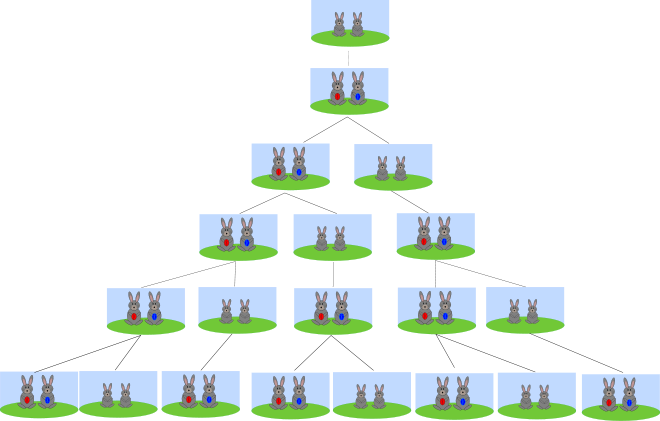
\includegraphics[width=0.6\textwidth]{fibonacci.png}
\end{center}

Cette suite est définie de la façon suivante : 

\begin{align*}
\left\{
\begin{array}{c}
F_0=0\\
\\
F_1=1\\
\\
F_{n+2}=F_{n+1}+F_{n}\\
\end{array}
\right.
\end{align*}





\question{Écriture sous Python \texttt{fib$\_$it(n:int)->F(n)} calculant le terme de rang $n$ ($F_n$) de la suite de Fibonacci par une méthode itérative. Donner la valeur de $F(n)$.}



\question{Écriture sous Python \texttt{fib$\_$rec(n:int)->F(n)} calculant le terme de rang $n$ ($F_n$) de la suite de Fibonacci par une méthode récursive naïve. Donner la valeur de $F(n)$.}


On donne les instruction suivantes qui permettent de compter le nombre d'appel à une fonction : 


\begin{lstlisting}
C=0
def compte_appel():
    global C
    C+=1

n=u(alpha,10)

for k in range(n):
    compte_appel()
\end{lstlisting}

\question{Exécuter cette suite d'instruction et donner la valeur de C dans votre cas.}



\question{En vous inspirant de la question précédente et avec la forme récursive Donner le nombre d'appel à la fonction \texttt{fib$\_$rec(n:int)->F(n)} par une méthode récursive "naïve" avec \texttt{n=u(alpha,10)}..}

Pour améliorer l'efficacité de la méthode, on va stocker chacun des termes dans une liste à chaque fois qu'il est calculé.

\question{Proposer un nouvelle fonction de signature \texttt{fib$\_$rec2(n:int)->int} en modifiant l'algorithme
précédent en y ajoutant la déclaration d'une liste. On ne calcule le n\up{ème} terme que si celui-ci n'a jamais été calculé. On pourra
commencer par déclarer une liste contenant n + 1 fois la valeur 0. Donner le nombre d'appel à la fonction \texttt{fib$\_$rec2(n:int)->F(n)} par cette méthode avec \texttt{n=u(alpha,10)}.}